\documentclass[12pt]{article}
\usepackage[a4paper, total={7.66in,  11.1in}]{geometry}
%\usepackage{array}
\usepackage{graphicx, subfig, wrapfig ,multicol, color,mathrsfs,mhchem, chemfig,fancyhdr,lastpage,float }
\setlength{\columnseprule}{1pt}
\def\columnseprulecolor{\color{blue}}
\usepackage[mathscr]{euscript}
\newcommand\headerMe[2]{\noindent{}#1\hfill#2}

\pagestyle{fancy}
\fancyhf{}
\cfoot{\vspace{-1cm}\em{Page:\thepage / \pageref{LastPage}}}

\begin{document}
\headerMe{Royaume du Maroc}{année scolaire \emph{2024-2025}}\\
\headerMe{Ministère de l'Éducation nationale, }{  Professeur :\emph{Zakaria Haouzan}}\\
\headerMe{du Préscolaire et des Sports}{Établissement : \emph{Lycée SKHOR qualifiant}}\\
\begin{center}
	\vspace{-0.8cm}
Evaluation Diagnostique \\
Filière Tronc Commun Scientifique\\
Durée 1h45
\\
 %   \vspace{.2cm}
%\hrulefill
%\Large{Chimie 6pts}
%\hrulefill\\
 %   \emph{Les deux parties sont indépendantes}
\end{center}
%end Headerss------------------------
\begin{center}
	\vspace{-0.2cm}
	\textbf{ Prénom.......................................  Nom.......................................}
	
	\vspace{0.2cm}
	\textbf{ Date.........................................  classe:................................... Note: }
		
\end{center}
\begin{center}

	\vspace{-0.55cm}
\underline{Consignes aux élèves : L’évaluation comporte 3 Parties: Mécanique,électronique et Chimie}

	\hrulefill
\textbf{Physique 70\%}
\hrulefill
\end{center}
%__________________Chimie ______________________-
%%%%%%%+_+_+_+_+_+_+_+_+_Partie1

\vspace{-1cm}
\begin{multicols}{2}
    [
	\section*{Partie 1 : Mécanique }
    ]

\begin{enumerate}

	\item \textbf{Répondre par VRAI ou par FAUX :} 
		\begin{enumerate}
			\item La masse est une grandeur fixe elle ne
				dépend pas du lieu. \dotfill
			\item La valeur de l’intensité du poids est une
 grandeur fixe elle dépond du lieu. \dotfill
\item Le poids est la force exercée par la terre
 sur un corps. \dotfill
\item La relation entre le poids et la masse est $P = \frac{m}{g}$ \dotfill
		\end{enumerate}
	\item \textbf{Répondre par VRAI ou par FAUX :} 
		\begin{enumerate}
			\item Dans un mouvement de translation la  trajectoire, d’un corps est une droite. \dotfill
\item Dans un mouvement rectiligne uniforme, la vitesse est constante.\dotfill
\item  La valeur de la vitesse augmente dans un
 mouvement rectiligne retardé. \dotfill
\item Dans un mouvement rectiligne uniforme
 la distance parcourue pendant les mêmes
 intervalles du temps est égales.\dotfill
		\end{enumerate}

%Exo 3
		\item \emph{La longueur d’une route traversant un village est $d$=$1000m$ , la vitesse limite qu’il ne faut pas
		dépasser par le conducteur est $V_{limite}$=$40Km/h$.
Le conducteur d’une voiture a mis la durée $t_1$=$100s$
pour traverser la distance $d$, par contre le conducteur d’un camion a mis $t_2$=$60s$. }  \textbf{ Calculez la vitesse moyenne pour chaque
conducteur en m/s et Km/h.}
\begin{enumerate}
	\item $V_{voiture}$ est: \dotfill
	\item $V_{camion}$ est : \dotfill
	\item Est ce que l’un des conducteurs a dépassé la
vitesse limite ?\dotfill
\end{enumerate}

\item \emph{Une boule de masse m=2.5Kg se trouve sur une table horizontale. On donne g=10N/Kg.}
	\textbf{L’intensité du poids est :}\dotfill
	\\\textbf{L’intensité de la force exercée par la table sur la boule est:}\dotfill
\item un corps (S) est en équilibre sous l’action de deux forces $\vec{F_1}$
et $\vec{F_2}$ si:
\begin{enumerate}
	\item $\vec{F_1}$ et $\vec{F_2}$ ont : même sens ,même intensité et même direction.

	\item $\vec{F_1}$ et $\vec{F_2}$  vérifient la relation suivante: $\vec{F_1}$+$\vec{F_2}$=$\vec{0}$.

	\item $\vec{F_1}$ et $\vec{F_2}$  vérifient la relation suivante: $F_1$+$F_2$=0.
\end{enumerate}

\begin{minipage}{\linewidth} 
\begin{wrapfigure}{r}{0.9in} 
\vspace{-12pt} 
\includegraphics[width=0.9in]{./img/dynamo.jpeg}
\vspace{-1cm}
\caption{}
\end{wrapfigure} 

\item \emph{La figure 1 représente un objet solide suspendu à un dynamomètre (verticale) par un fil inétendu dont sa masse est
négligeable. La figure  1 représente un
objet solide suspendu à un dynamomètre (verticale) par un fil
inétendu dont sa masse est négligeable.}

\end{minipage}
\begin{enumerate}
	\item Son poids est P=\dotfill
	\item Sa direction est\dotfill
\end{enumerate}
\item Quand la vitesse d’un objet est constante, le mouvement est dit
	\begin{enumerate}
		\item Accéléré
		\item Ralenti
		\item Uniforme
	\end{enumerate}

\end{enumerate}

\end{multicols}
 %Parte 2 électronique : 
\vspace{0.8cm}
\begin{multicols}{2}
    [
	\section*{\begin{center}\underline{Partie 2 :  électronique }\end{center}}
    ]
	\begin{enumerate}

\begin{minipage}{\linewidth} 
\begin{wrapfigure}{r}{1.3in} 
\vspace{-12pt} 
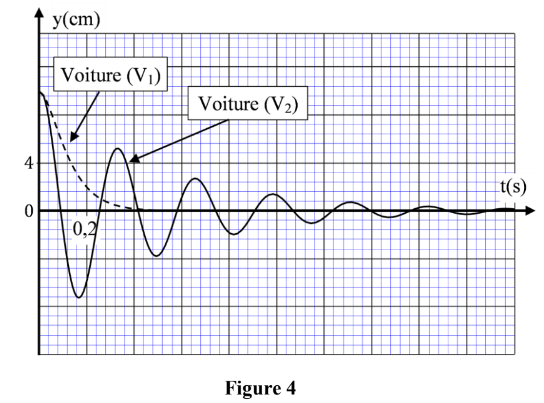
\includegraphics[width=1.3in]{./img/oscillo.png}
%\vspace{-1cm}
\caption{}
\end{wrapfigure} 


		\item Le schéma suivant représente la tension aux bornes d’un conducteur ohmique lorsqu’on le visualise avec un oscilloscope . la résistance du conducteur ohmique est $R$=$6\Omega$.la sensibilité verticale est 5V/div.
\textbf{Répondre par VRAI ou par FAUX :}
		\end{minipage}
		\begin{enumerate}
		\item la tension aux bornes du conducteur ohmique est 30V.\dotfill
		\item la tension aux bornes du conducteur ohmique est 60V.\dotfill
		\item La tension aux bornes du conducteur ohmique est alternative et sinusoïdale.\dotfill
		\item L’intensité du courant traversant le conducteur est I=0.5A\dotfill
		\end{enumerate}

	\item Quelle est l'intensité efficace du courant traversant
d'une lampe lorsqu'elle est branchée sur le
secteur? (P = 75 W) et U = 230 V 
\begin{enumerate}
	\item $I_{eff} = 0,33A$
	\item $I_{eff} = 17250A$
	\item $I_{eff} = 3,1A$
\end{enumerate}
\item Une lampe de phare d'un automibile a une puissance de 45 W. l'énergie consommé par la lampe pour une durée de fonctionnement
de 3H
\begin{enumerate}
	\item E= 15J
	\item E= 135J
	\item E= 135Wh
\end{enumerate}
\item Donner les unités pour la formule de l'énergie
électrique consommée par un appareil 
\begin{enumerate}
	\item  E en Wh, P en W et t en s
	\item E en J, P en W et t en s 
	\item  E en J , P en W et t en h
\end{enumerate}

\begin{minipage}{\linewidth} 
\begin{wrapfigure}{r}{2.2in} 
\vspace{-1cm} 
\includegraphics[width=2.2in]{./img/Resistance.png}
%\caption{}
\end{wrapfigure} 


\item D’après le graphique ci-contre qui donne la caractéristique d’un dipôle,
\end{minipage}
\begin{enumerate}
	\vspace{0.5cm}

	\item Déterminer graphiquement la valeur de la résistance utilisée R=\dotfill
\end{enumerate}
\item Dans un circuit en série, quand on ajoute une résistance, alors l'intensité du courant
	\begin{enumerate}
		\item augmente
		\item diminue
		\item reste la même.
	\end{enumerate}
\item Dans les appareils de chauffage, une résistance permet de produire 
	\begin{enumerate}
		\item du courant électrique
		\item de l'énergie solaire
		\item de la chaleur
	\end{enumerate}
\item L’énergie consommée par un appareil de chauffage est donnée par :
	\begin{enumerate}
		\item $E=R.I^2.t$
		\item $E=R.I.t$
		\item $E=U.I^2.t$
	\end{enumerate}
\item La relation de la puissance électrique reçue par un appareil en courant continu est
	\begin{enumerate}
		\item $P=\frac{U}{I}$
		\item $U=\frac{I}{P}$
		\item $P=U.I$
	\end{enumerate}
\item Une lampe porte l’indication (6V-1,8W) ; en fonctionnement en sous-tension, l’intensité du
courant vaut- elle ?:
\begin{enumerate}
	\item I=0,3A
	\item I=0,18A
	\item I=0,6A
\end{enumerate}


	\end{enumerate}
\end{multicols}	



\begin{center}

\vspace{4cm}
\hrulefill
\textbf{Chimie 30\%}
\hrulefill


\end{center}
\begin{multicols}{2}
    [
        \section*{Partie 3 :Chimie}
    ]
	\begin{enumerate}
		\item Pour savoir si un morceau de pain contient de l’eau, on utilise l’espèce
chimique suivante :
\begin{enumerate}
	\item le sulfate de cuivre
	\item le sulfate de cuivre anhydre
	\item l’eau iodée
	\item l’eau de chaux
\end{enumerate}
\item Pour obtenir simplement une eau limpide à partir d’une eau boueuse, on
peut réaliser l’expérience schématisée ci-contre. Il s’agit
d’une:
\begin{enumerate}
	\item distillation
	\item filtration
	\item décantation
\end{enumerate}

\begin{minipage}{\linewidth} 
\begin{wrapfigure}{r}{1.8in} 
\vspace{-12pt} 
\includegraphics[width=1.8in]{./img/filtration.png}
\vspace{-1cm}
\caption{}
\end{wrapfigure} 

\item Donner le numéro correspondant aux termes suivants (Figure 3):

\end{minipage}
	\begin{enumerate}
		\item  Support:N°...
		\item  Entonnoir:N°...
		\item  Filtrat:N°...
		\item  Mélange hétérogène:N°...
		\item  Filtre:N°...
		\item  Baguette:N°...
	\end{enumerate}
\item Dans un aquarium, le pH de l’eau doit se situer entre 6,5 et 7,5. Lors d’un contrôle, on a relevé la mesure suivante : pH = 8,2. \textbf{Indique si l’eau est plutôt :}
	\begin{enumerate}
		\item  Acide
		\item  Neutre
		\item  Basique
	\end{enumerate}
\item Lorsqu'on dilue une solution acide, le PH de cette solution :
	\begin{enumerate}
		\item reste constante
		\item augmente
		\item diminue
		\end{enumerate}
	\item La charge de l’ion $Al^{3+}$ est:
		\begin{enumerate}
			\item q=-3e
			\item $q=1,6.10^{-19}C$
			\item q=+3e
		\end{enumerate}
	\item Les matériaux organiques sont composés principalement de :
		\begin{enumerate}
			\item le Carbone et le Fer
			\item le Carbone et l’hydrogène
			\item le Carbone et l’Oxygène.
		\end{enumerate}
	\item Les constituants de l’atome sont : 
		\begin{enumerate}
			\item Les électrons et le noyau
			\item Les électrons
			\item Les ions et les électrons
			\item Les électrons et les ions
		\end{enumerate}
	\item Une casserole en cuivre est remplie avec 5L d'eau salée ( $\rho$=$1.14 g/cm^3$ ). La casserole remplie a une masse de 8kg . Détermine la masse en cuivre utilisé pour fabriquer la casserole.
		\begin{enumerate}
	\item m = 5,7 Kg
	\item m = 1,14 Kg
	\item m = 2,3 Kg
	\end{enumerate}
	\end{enumerate}
\end{multicols}











%%%%%%%+_+_+_+_+_+_+_+_+_Partie2
%________________________________________
\end{document}
